\chapter{Eletrostática: o campo e a lei de Gauss}\label{ch:b1:electrostatics-gauss}

Esfregue um balão num suéter e ele gruda na parede; penteie um cabelo seco
e o pente entorta um filete fino de água. Por trás dos dois está a força
entre \omterm{def:b1:electrostatics-gauss:charge}{cargas elétricas} em repouso, a \omterm{thm:b1:electrostatics-gauss:coulomb}{lei de Coulomb} --- uma lei em inverso
do quadrado como a \omterm{def:b1:central-forces:gravitation}{gravitação}, mas $10^{36}$ vezes mais forte entre dois
prótons e com os dois sinais, de modo que a matéria é neutra com precisão
fantástica e os efeitos residuais são o que chamamos de química, materiais e
raios. Este capítulo constrói o conceito que torna a lei manejável, o \omterm{def:b1:electrostatics-gauss:field}{campo
elétrico}, mostra como ler um campo a partir das suas simetrias e deduz o
único teorema que calcula em três linhas os campos de distribuições
simétricas: a \omterm{thm:b1:electrostatics-gauss:gauss}{lei de Gauss}. O seu gêmeo gravitacional vem de brinde no fim.

\begin{omfigure}
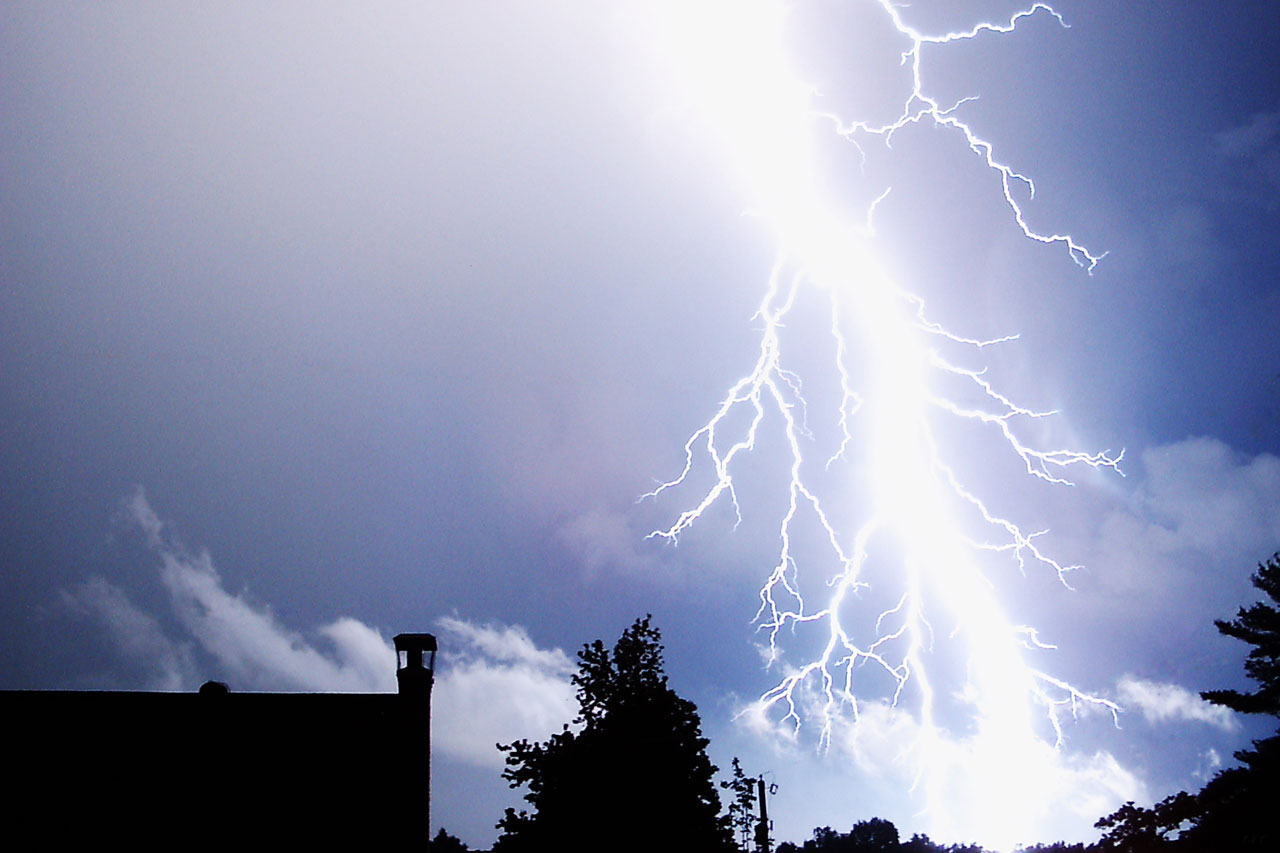
\includegraphics[width=0.50\linewidth]{images/book3/lightning-strike.jpg}

{\small Um raio de nuvem para o solo: dezenas de coulombs trazidos para baixo em algumas descargas de cem quiloampères --- a Terra elétrica do problema de fim de semana.}
\end{omfigure}

\section{Cargas e a lei de Coulomb}

\begin{definition}[Carga elétrica]\label{def:b1:electrostatics-gauss:charge}
\index{carga elétrica}\index{carga elementar}\index{densidade de carga}
A \emph{carga elétrica} $q$ (coulomb, \unit{C}) é uma propriedade da
matéria, dos dois sinais; ela se conserva (a carga total de um sistema
isolado nunca muda) e é quantizada em unidades da \emph{carga elementar}
$e = \qty{1.602e-19}{C}$ (próton $+e$, elétron $-e$). Uma distribuição
macroscópica é descrita por uma \emph{densidade de carga}: linear $\lambda$
(\unit{C/m}), superficial $\sigma$ (\unit{C/m^2}) ou volumétrica $\rho$
(\unit{C/m^3}), de modo que um pequeno elemento leva $\dd q = \lambda\,\dd l$,
$\sigma\,\dd S$ ou $\rho\,\dd\tau$.
\end{definition}

\begin{theorem}[Lei de Coulomb]\label{thm:b1:electrostatics-gauss:coulomb}
\index{lei de Coulomb}\index{permissividade do vácuo}
Duas cargas pontuais $q_1$ em $M_1$ e $q_2$ em $M_2$ em repouso no vácuo
exercem uma sobre a outra as forças
\[
\vect F_{1 \to 2} = \frac{q_1q_2}{4\pi\varepsilon_0\,r^2}\,\vect e_{12} = -\vect F_{2 \to 1},
\qquad r = M_1M_2,\quad \vect e_{12} = \frac{\vect{M_1M_2}}{r},
\]
repulsivas para cargas de mesmo sinal e atrativas para cargas de sinais
contrários, com a \emph{\omterm{thm:b1:electrostatics-gauss:coulomb}{permissividade do vácuo}} $\varepsilon_0 = \qty{8.854e-12}{F/m}$, isto é,
$1/4\pi\varepsilon_0 = \qty{8.99e9}{N.m^2/C^2}$. As forças de várias cargas se somam
(superposição).
\end{theorem}
\admitted

\begin{example}[Quão forte]\label{ex:b1:electrostatics-gauss:strong}
Dois prótons a \qty{1}{fm} um do outro se repelem com $8.99 \times 10^9 \times (1.6 \times
10^{-19})^2/10^{-30} = \qty{230}{N}$ --- o peso de uma criança, entre duas
partículas de $10^{-27}$~kg; a atração gravitacional entre eles é
$10^{36}$ vezes menor. Dois gramas de elétrons numa ponta de uma sala
e os prótons correspondentes na outra se atrairiam com $10^{25}$~N.
A matéria é neutra porque não tem escolha: qualquer desequilíbrio é corrigido
por forças que estrutura nenhuma resiste.
\end{example}

\section{O campo elétrico}

\begin{definition}[Campo eletrostático]\label{def:b1:electrostatics-gauss:field}
\index{campo elétrico}\index{linha de campo}
Uma distribuição de cargas em repouso cria em todo ponto $M$ do espaço
um \emph{campo elétrico} $\vect E(M)$, definido pela força que ele exerce sobre
uma carga de prova $q$ colocada em $M$: $\vect F = q\vect E(M)$ (\unit{V/m} $=$
\unit{N/C}). Uma carga pontual $q_1$ em $O$ cria
\[
\vect E(M) = \frac{q_1}{4\pi\varepsilon_0 r^2}\,\vect e_r , \qquad r = OM ,
\]
radial e para fora se $q_1 > 0$; uma distribuição cria a soma vetorial dos
campos dos seus elementos. Uma \emph{linha de campo} é uma curva tangente em
cada ponto a $\vect E$, orientada segundo ele.
\end{definition}

\begin{proposition}[Ler um mapa de campo]\label{prop:b1:electrostatics-gauss:lines}
As \omterm{def:b1:electrostatics-gauss:field}{linhas de campo} saem das cargas positivas e terminam nas negativas (ou
no infinito); elas nunca se cruzam (o campo é unívoco) e se adensam onde
o campo é forte. Quando há duas cargas presentes, o
número de linhas desenhadas em cada uma é proporcional à sua carga.
\end{proposition}

\begin{omfigure}
\begin{tikzpicture}[font=\small, x=1cm, y=1cm, >=Stealth]
  % dipole: arcs through (-1,0) and (1,0), centre (0,c)
  \begin{scope}[scale=1.4]
    \foreach \c in {0.1, 0.55, 1.6} {
      \draw[omDef, thick, postaction={decorate, decoration={markings, mark=at position 0.5 with {\arrow{>}}}}]
        let \n1 = {sqrt(1+\c*\c)} in
        (-1,0) arc[start angle={180+atan2(\c,1)}, end angle={360-atan2(\c,1)}, radius=\n1 cm];
      \draw[omDef, thick, postaction={decorate, decoration={markings, mark=at position 0.5 with {\arrow{>}}}}]
        let \n1 = {sqrt(1+\c*\c)} in
        (-1,0) arc[start angle={180-atan2(\c,1)}, end angle={atan2(\c,1)}, radius=\n1 cm];
    }
    \draw[omDef, thick, postaction={decorate, decoration={markings, mark=at position 0.5 with {\arrow{>}}}}] (-1,0) -- (1,0);
    \draw[omDef, thick, postaction={decorate, decoration={markings, mark=at position 0.6 with {\arrow{>}}}}] (-2.6,0) -- (-1,0);
    \draw[omDef, thick, postaction={decorate, decoration={markings, mark=at position 0.4 with {\arrow{>}}}}] (1,0) -- (2.6,0);
    \fill[omThm] (-1,0) circle (3pt) node[below left] {$+q$};
    \fill[omDef] (1,0) circle (3pt) node[below right] {$-q$};
  \end{scope}
  % two like charges
  \begin{scope}[xshift=7.9cm, fl/.style={omThm, thick, postaction={decorate, decoration={markings, mark=at position 0.55 with {\arrow{>}}}}}]
    \foreach \s in {1,-1} {
      % left charge at (-1,0), right charge at (1,0); \s mirrors up/down
      \draw[fl] (-1,0) -- (-3.4,0);
      \draw[fl] (1,0) -- (3.4,0);
      \draw[fl] (-1,0) .. controls (-2.2,{1.2*\s}) .. (-3.2,{2.0*\s});
      \draw[fl] (1,0) .. controls (2.2,{1.2*\s}) .. (3.2,{2.0*\s});
      \draw[fl] (-1,0) .. controls (-1.1,{1.3*\s}) .. (-1.6,{2.9*\s});
      \draw[fl] (1,0) .. controls (1.1,{1.3*\s}) .. (1.6,{2.9*\s});
      \draw[fl] (-1,0) .. controls (-0.2,{0.7*\s}) and (-0.1,{1.6*\s}) .. (-0.3,{2.9*\s});
      \draw[fl] (1,0) .. controls (0.2,{0.7*\s}) and (0.1,{1.6*\s}) .. (0.3,{2.9*\s});
    }
    \draw[fl] (-1,0) -- (-0.08,0);
    \draw[fl] (1,0) -- (0.08,0);
    \fill[omThm] (-1,0) circle (3pt) node[below left] {$+q$};
    \fill[omThm] (1,0) circle (3pt) node[below right] {$+q$};
    \fill (0,0) circle (1.2pt) node[below, font=\footnotesize, yshift=-2pt] {$\vect E = \vect 0$};
  \end{scope}
\end{tikzpicture}

{\small \omterm{def:b1:electrostatics-gauss:field}{Linhas de campo} de duas cargas opostas (à esquerda) e de duas
cargas positivas iguais (à direita). As linhas partem do $+$ e terminam no
$-$ ou no infinito; à direita elas se repelem e o campo se anula no
ponto médio, por onde não passa nenhuma linha.}
\end{omfigure}

\begin{example}[Anel e segmento por soma direta]\label{ex:b1:electrostatics-gauss:ring}
No eixo de um anel de raio $R$ que leva $Q$ uniformemente, à distância
$z$ do seu centro, cada elemento $\dd q$ contribui com $\dd q/4\pi\varepsilon_0(R^2 +
z^2)$ ao longo da reta que o liga a $M$; as componentes perpendiculares
ao eixo se cancelam aos pares e as axiais se somam com o fator
$z/\sqrt{R^2 + z^2}$:
\[
E_z = \frac{Qz}{4\pi\varepsilon_0(R^2 + z^2)^{3/2}} ,
\]
nulo no centro, máximo em $z = R/\sqrt2$ e igual a $Q/4\pi\varepsilon_0z^2$ bem
longe. Um disco carregado uniformemente é uma pilha de anéis (\cref{pb:b1:electrostatics-gauss:1}).
A soma direta funciona sempre que a geometria permite calcular a integral; o
resto do capítulo trata de evitá-la.
\end{example}

\section{Simetrias e invariâncias}

\begin{proposition}[Princípio de simetria]\label{prop:b1:electrostatics-gauss:symmetry}
\index{simetria (de um campo)}\index{plano de simetria}\index{plano de antissimetria}
O campo tem as simetrias das suas fontes. Se um plano $\Pi$ é um
\emph{\omterm{prop:b1:electrostatics-gauss:symmetry}{plano de simetria}} da distribuição de cargas (a imagem especular
da distribuição é ela própria), então em todo ponto de $\Pi$ o campo
está \emph{contido} em $\Pi$; se $\Pi$ é um \emph{\omterm{prop:b1:electrostatics-gauss:symmetry}{plano de antissimetria}}
(a imagem especular é a distribuição com todas as cargas trocadas de sinal), o
campo nos pontos de $\Pi$ é \emph{perpendicular} a $\Pi$. Se a
distribuição é invariante por uma translação ou por uma rotação, o campo
também é: as suas componentes não dependem da coordenada correspondente.
\end{proposition}

\begin{proof}
$\vect E$ é uma soma de termos $\dd q\,\vect e/4\pi\varepsilon_0r^2$; a imagem
especular da soma é a soma das imagens, e a imagem do campo
de uma distribuição é o campo da distribuição imagem (um vetor
construído a partir de posições e cargas se transforma como as posições). Num
\omterm{prop:b1:electrostatics-gauss:symmetry}{plano de simetria} o campo é igual à sua própria imagem especular e portanto está no
plano; num \omterm{prop:b1:electrostatics-gauss:symmetry}{plano de antissimetria} ele é igual ao oposto da sua imagem e
portanto é normal a ele. A invariância é o mesmo argumento com uma
translação ou uma rotação.
\end{proof}

\begin{method}[Achar a forma de um campo antes de calculá-lo]\label{meth:b1:electrostatics-gauss:symmetry}
Para o ponto $M$ em que se quer o campo: (1) liste os \omterm{prop:b1:electrostatics-gauss:symmetry}{planos de
simetria} das fontes que contêm $M$ --- o campo está sobre a interseção
deles; dois desses planos fixam a direção. (2) Liste as
invariâncias --- elas dizem de que coordenadas $\vect E$ depende. Assim, um
fio infinito carregado uniformemente dá $\vect E = E(r)\,\vect e_r$ em
\omterm{def:b1:point-kinematics:cylindrical}{coordenadas cilíndricas}, uma esfera dá $\vect E = E(r)\,\vect e_r$ em
esféricas, e um plano infinito dá $\vect E = E(z)\,\vect e_z$ com $E(-z) = -E(z)$.
Só então calcule.
\end{method}

\begin{omfigure}
\begin{tikzpicture}[font=\small, x=1cm, y=1cm, >=Stealth]
  % sphere
  \begin{scope}
    \draw[omDef, fill=omDef!15] (0,0) circle (0.9);
    \draw[dashed] (0,0) circle (1.8);
    \foreach \a in {0,45,...,315} \draw[omThm, thick, ->] (\a:1.8) -- ++(\a:0.6);
    \node[font=\footnotesize] at (0,-2.75) {$\vect E = E(r)\,\vect e_r$};
    \node[font=\footnotesize, omDef] at (0,0) {$Q$};
  \end{scope}
  % cylinder / wire
  \begin{scope}[xshift=5.2cm]
    \draw[omDef, very thick] (0,-2.2) -- (0,2.2) node[above, font=\footnotesize] {$\lambda$};
    \draw[dashed] (-1.1,-1.6) rectangle (1.1,1.6);
    \draw[dashed] (0,1.6) ellipse (1.1 and 0.28);
    \draw[dashed] (0,-1.6) ellipse (1.1 and 0.28);
    \foreach \y in {-1.0,-0.3,0.4,1.1} {\draw[omThm, thick, ->] (1.1,\y) -- ++(0.6,0); \draw[omThm, thick, ->] (-1.1,\y) -- ++(-0.6,0);}
    \node[font=\footnotesize] at (0,-2.75) {$\vect E = E(r)\,\vect e_r$ (cilíndricas)};
  \end{scope}
  % plane
  \begin{scope}[xshift=10.4cm]
    \draw[omDef, fill=omDef!25] (-1.8,-0.25) -- (1.8,-0.25) -- (2.2,0.25) -- (-1.4,0.25) -- cycle;
    \node[omDef, font=\footnotesize] at (1.9,-0.45) {$\sigma$};
    \draw[dashed] (-0.5,-1.4) rectangle (0.5,1.4);
    \foreach \x in {-1.2,0,1.2} {\draw[omThm, thick, ->] (\x,0.35) -- ++(0,0.9); \draw[omThm, thick, ->] (\x,-0.35) -- ++(0,-0.9);}
    \node[font=\footnotesize] at (0,-2.75) {$\vect E = E(z)\,\vect e_z$, ímpar em $z$};
  \end{scope}
\end{tikzpicture}

{\small As três distribuições simétricas do capítulo e as
superfícies de Gauss (tracejadas) adaptadas a elas: uma esfera concêntrica, um
cilindro coaxial e uma caixinha cilíndrica atravessando o plano. Em cada uma, o campo é
normal e de módulo uniforme, ou então tangente.}
\end{omfigure}

\section{Fluxo e lei de Gauss}

\begin{definition}[Fluxo do campo]\label{def:b1:electrostatics-gauss:flux}
\index{fluxo do campo elétrico}
Corte uma superfície $S$ em pequenos elementos de área $\dd S$, cada um com uma
normal unitária $\vect n$ (para uma superfície fechada, a normal para fora). O
\emph{fluxo} de $\vect E$ através de $S$ é a soma
\[
\Phi = \sum \vect E\cdot\vect n\,\dd S = \sum E_n\,\dd S \qquad (\unit{V.m}):
\]
a componente normal do campo ponderada pela área --- o ``número de \omterm{def:b1:electrostatics-gauss:field}{linhas de
campo}'' que atravessam $S$, contadas positivamente quando cruzam no sentido de
$\vect n$.
\end{definition}

\begin{theorem}[Lei de Gauss]\label{thm:b1:electrostatics-gauss:gauss}
\index{lei de Gauss}
O \omterm{def:b1:electrostatics-gauss:flux}{fluxo} do campo eletrostático através de qualquer superfície fechada $S$
é igual à carga total encerrada por $S$ dividida por $\varepsilon_0$:
\[
\Phi_{\text{saída}} = \frac{Q_{\text{int}}}{\varepsilon_0} .
\]
As cargas fora de $S$ não contribuem em nada para o \omterm{def:b1:electrostatics-gauss:flux}{fluxo} (as suas linhas entram
e voltam a sair).
\end{theorem}

\begin{proof}
Para uma carga pontual $q$ no centro de uma esfera de raio $r$:
$\vect E$ é radial, de módulo $q/4\pi\varepsilon_0r^2$ em toda a
esfera, logo $\Phi = E \times 4\pi r^2 = q/\varepsilon_0$ --- independente de $r$,
porque o campo cai como $1/r^2$ exatamente na medida em que a área cresce. Que o
mesmo valha para qualquer superfície fechada em torno de $q$ (o \omterm{def:b1:electrostatics-gauss:flux}{fluxo} através de um
elemento de superfície só depende do ângulo sólido que ele subtende desde $q$),
que uma carga externa dê zero (ela subtende duas vezes cada ângulo sólido,
com sinais opostos) e que os \omterm{def:b1:electrostatics-gauss:flux}{fluxos} de várias cargas se somem fica
admitido aqui; a demonstração completa está no volume do segundo ano.
\end{proof}

\begin{method}[Usar a lei de Gauss]\label{meth:b1:electrostatics-gauss:gauss}
(1) A partir das simetrias, escreva a forma de $\vect E$ (direção e a
variável de que ele depende). (2) Escolha uma \emph{superfície de Gauss} fechada
que passe pelo ponto $M$ e na qual $\vect E$ seja em toda parte normal com
o mesmo módulo $E(M)$, ou então tangente: o \omterm{def:b1:electrostatics-gauss:flux}{fluxo} é então $E(M)$ vezes a
área da parte normal. (3) Conte a carga que está dentro. (4) Isole
$E(M)$. Funciona para esferas, cilindros infinitos e planos infinitos
--- e para nada mais, sem outras ferramentas.
\end{method}

\begin{proposition}[Os três campos clássicos]\label{prop:b1:electrostatics-gauss:three}
\index{campo de uma esfera carregada}\index{campo de um fio carregado}\index{campo de um plano carregado}
\begin{enumerate}
  \item Esfera de raio $R$, de carga $Q$ espalhada uniformemente no seu
        volume: $E(r) = \dfrac{Q}{4\pi\varepsilon_0r^2}$ fora ($r > R$) ---
        como se toda a carga estivesse no centro --- e $E(r) =
        \dfrac{Qr}{4\pi\varepsilon_0R^3}$ dentro, crescendo linearmente a partir de zero;
        contínuo em $r = R$. Se a carga estiver só na superfície,
        o campo interno é nulo.
  \item Fio infinito de carga linear $\lambda$: $E(r) =
        \dfrac{\lambda}{2\pi\varepsilon_0 r}$, radial.
  \item Plano infinito de carga superficial $\sigma$: $E = \dfrac{\sigma}{2\varepsilon_0}$
        de cada lado, normal ao plano, apontando para longe dele se
        $\sigma > 0$, \emph{independentemente da distância}. Ao atravessar o plano
        a componente normal salta de $\sigma/\varepsilon_0$.
\end{enumerate}
\end{proposition}

\begin{proof}
(1) Esfera de raio $r$: \omterm{def:b1:electrostatics-gauss:flux}{fluxo} $4\pi r^2E(r)$; carga interna $Q$ se
$r > R$, e $Q(r/R)^3$ se $r < R$. (2) Cilindro de raio $r$ e comprimento $h$:
\omterm{def:b1:electrostatics-gauss:flux}{fluxo} pela superfície lateral $2\pi rh\,E(r)$, nenhum pelas bases
(campo tangente); carga $\lambda h$. (3) Caixinha cilíndrica de seção $S$
atravessando o plano: \omterm{def:b1:electrostatics-gauss:flux}{fluxo} $2SE$ pelas duas bases (o campo é ímpar
em $z$, de modo que as duas contam positivamente), nenhum pela lateral; carga
$\sigma S$.
\end{proof}

\begin{omfigure}
\begin{tikzpicture}
\begin{axis}[omaxis, axis x line=bottom, axis y line=left, width=10cm, height=5.6cm,
    xlabel={$r/R$}, ylabel={$E$ (em unidades de $Q/4\pi\varepsilon_0R^2$)},
    xlabel style={at={(axis description cs:0.5,-0.1)}, anchor=north},
    xmin=0, xmax=4, ymin=0, ymax=1.3, xtick={1,2,3}, ytick={0.5,1}, samples=80]
  \addplot[omDef, very thick, domain=0:1] {x} node[pos=0.85, above left, font=\footnotesize] {volume: $\propto r$};
  \addplot[omDef, very thick, domain=1:4] {1/x^2} node[pos=0.35, above right, font=\footnotesize] {$\propto 1/r^2$};
  \addplot[omThm, thick, dashed] coordinates {(0,0) (1,0)};
  \addplot[omThm, thick, dashed] coordinates {(1,0) (1,1)};
  \node[omThm, font=\footnotesize, anchor=west] at (axis cs:1.08,0.08) {superfície: $0$ dentro};
\end{axis}
\end{tikzpicture}

{\small O \omterm{prop:b1:electrostatics-gauss:three}{campo de uma esfera carregada} em função da distância ao seu centro:
linear dentro e em $1/r^2$ fora quando a carga preenche o volume
(traço cheio); nulo dentro e o mesmo fora quando ela está na superfície
(tracejado). Do lado de fora, nada distingue a esfera de uma carga pontual
no seu centro.}
\end{omfigure}

\begin{example}[Dois planos: o capacitor plano]\label{ex:b1:electrostatics-gauss:twoplanes}
\index{capacitor plano!campo}
Dois planos paralelos que levam $+\sigma$ e $-\sigma$: cada um cria
$\sigma/2\varepsilon_0$ apontando para longe de si (em direção a si, no caso do negativo).
Entre os planos os dois campos se somam e dão $\sigma/\varepsilon_0$, dirigido do
$+$ para o $-$; fora eles se cancelam. Com $\sigma = \qty{1}{\micro C/m^2}$, $E =
10^{-6}/8.85 \times 10^{-12} = \qty{1.1e5}{V/m}$ entre eles e zero fora: o
campo de um capacitor carregado fica confinado ao seu espaçamento
(\cref{ch:b1:potential-capacitors}).
\end{example}

\begin{omfigure}
\begin{tikzpicture}[font=\small, x=1cm, y=1cm, >=Stealth]
  \draw[omThm, very thick] (-0.8,-2) -- (-0.8,2) node[above] {$+\sigma$};
  \draw[omDef, very thick] (0.8,-2) -- (0.8,2) node[above] {$-\sigma$};
  % field of + plane (red), of - plane (blue), resultant (black)
  \foreach \y in {-1.4,-0.7,0,0.7,1.4} {
    \draw[omThm, ->] (-0.8,\y) -- ++(0.55,0);
    \draw[omThm, ->] (-0.8,\y) -- ++(-0.55,0);
    \draw[omDef, ->] (0.8,\y) -- ++(-0.55,0);
    \draw[omDef, ->] (0.8,\y) -- ++(0.55,0);
  }
  \node[omThm, font=\footnotesize, anchor=east] at (-1.0,-2.4) {só $+\sigma$: $\sigma/2\varepsilon_0$};
  \node[omDef, font=\footnotesize, anchor=west] at (1.0,-2.4) {só $-\sigma$: $\sigma/2\varepsilon_0$};
  \begin{scope}[xshift=7.2cm]
    \draw[omThm, very thick] (-0.8,-2) -- (-0.8,2) node[above] {$+\sigma$};
    \draw[omDef, very thick] (0.8,-2) -- (0.8,2) node[above] {$-\sigma$};
    \foreach \y in {-1.4,-0.7,0,0.7,1.4} \draw[black, very thick, ->] (-0.75,\y) -- (0.7,\y);
    \node[font=\footnotesize] at (0,-2.4) {total: $\sigma/\varepsilon_0$ entre, $0$ fora};
  \end{scope}
\end{tikzpicture}

{\small Superposição para duas folhas opostas. À esquerda: os campos
uniformes de cada folha isolada (em vermelho, o da positiva; em azul, o
dirigido à negativa). À direita: a sua soma, $\sigma/\varepsilon_0$ no espaçamento e zero fora.}
\end{omfigure}

\section{A analogia gravitacional}

\begin{proposition}[Lei de Gauss para a gravitação]\label{prop:b1:electrostatics-gauss:gravity}
\index{lei de Gauss!para a gravitação}\index{campo gravitacional}
A lei de Newton $\vect F = -Gm_1m_2\,\vect e_{12}/r^2$ tem a forma da de
Coulomb com $q \to m$ e $1/4\pi\varepsilon_0 \to -G$. O \omterm{prop:b1:newton-dynamics:weight}{campo gravitacional}
$\vect g$ (força por unidade de massa) obedece, portanto, às mesmas regras de
simetria e a
\[
\Phi_{\text{saída}}(\vect g) = -4\pi G\,M_{\text{int}} .
\]
Em particular, um corpo de simetria esférica atrai os pontos externos como
se a sua massa estivesse no seu centro, e o campo dentro de uma esfera homogênea
de raio $R$ e massa $M$ vale $g(r) = GMr/R^3$, linear em $r$.
\end{proposition}

\begin{proof}
Substitua $Q/\varepsilon_0$ por $-4\pi GM$ na demonstração da
\cref{prop:b1:electrostatics-gauss:three}; o sinal de menos diz que o \omterm{def:b1:electrostatics-gauss:flux}{fluxo}
entra (a gravidade atrai).
\end{proof}

\begin{example}[Dentro da Terra]\label{ex:b1:electrostatics-gauss:earth}
Numa Terra homogênea, $g$ cairia linearmente de \qty{9.8}{m/s^2} na
superfície até zero no centro; uma pedra solta num túnel que atravessasse
o planeta oscilaria harmonicamente com período $2\pi\sqrt{R/g} =
\qty{84}{min}$ --- o período de um satélite rasante. A Terra real tem
um núcleo denso, e $g$ de fato \emph{sobe} até \qty{10.7}{m/s^2} na
fronteira núcleo--manto antes de cair (\cref{pb:b1:electrostatics-gauss:1}).
Newton precisou do teorema das cascas para aplicar a sua lei aos planetas; a \omterm{thm:b1:electrostatics-gauss:gauss}{lei de
Gauss} o dá numa linha.
\end{example}

\section{Exercícios}

\begin{exercise}[$\star$]\label{exo:b1:electrostatics-gauss:1}
Força elétrica e força gravitacional entre dois prótons a
\qty{2.0}{fm} um do outro; a razão entre elas. Por que, então, os núcleos se mantêm coesos?
\end{exercise}

\begin{exercise}[$\star$]\label{exo:b1:electrostatics-gauss:2}
Campo a \qty{1.0}{m} de uma carga pontual de \qty{1.0}{\micro C}. A superfície
da Terra tem um campo de \qty{100}{V/m} apontando para baixo: sinal e valor da
carga da Terra, tratando-a como uma esfera de raio \qty{6370}{km}.
\end{exercise}

\begin{exercise}[$\star$]\label{exo:b1:electrostatics-gauss:3}
Duas cargas $+q$ em $x = \pm a$ no eixo $x$. Campo no eixo $x$
para $|x| > a$ e no eixo $y$; mostre que no eixo $y$ o $E_y$ é
máximo em $y = a/\sqrt2$. Esboce as linhas perto da origem.
\end{exercise}

\begin{exercise}[$\star$]\label{exo:b1:electrostatics-gauss:4}
Cargas $+2q$ em $x = 0$ e $-q$ em $x = a$. Onde o campo se anula no
eixo $x$? Quantas \omterm{def:b1:electrostatics-gauss:field}{linhas de campo} saem de $+2q$ para cada uma que
chega em $-q$, e para onde vão as outras?
\end{exercise}

\begin{exercise}[$\star\star$]\label{exo:b1:electrostatics-gauss:5}
Um disco de raio $R$ leva $\sigma$ uniformemente. A partir do resultado do anel,
mostre que no seu eixo $E_z = \dfrac{\sigma}{2\varepsilon_0}\Bigl(1 - \dfrac{z}{\sqrt{z^2 +
R^2}}\Bigr)$ para $z > 0$; verifique os dois limites $z \ll R$ e $z \gg R$.
\end{exercise}

\begin{exercise}[$\star\star$]\label{exo:b1:electrostatics-gauss:6}
Um núcleo de ouro ($Z = 79$, $R = \qty{7.0}{fm}$) como esfera carregada
uniformemente: campo na superfície, em $R/2$ e a \qty{1}{pm}. Compare com o
campo de ruptura do ar, \qty{3e6}{V/m}.
\end{exercise}

\begin{exercise}[$\star\star$]\label{exo:b1:electrostatics-gauss:7}
Campo de um fio infinito pela \omterm{thm:b1:electrostatics-gauss:gauss}{lei de Gauss}. Um condutor de alta \omterm{def:b1:dc-circuits:voltage}{tensão} de
raio \qty{1.0}{cm}: carga linear com que o campo na sua superfície
atinge o valor de ruptura \qty{3e6}{V/m} (início do efeito corona). Campo a
\qty{5}{m} nesse caso.
\end{exercise}

\begin{exercise}[$\star\star$]\label{exo:b1:electrostatics-gauss:8}
Duas placas paralelas de área \qty{1.0}{m^2} levam $\pm\qty{1.0}{\micro C}$.
Campo entre elas; força sobre uma das placas (o campo que age sobre ela é o
da outra placa apenas --- por quê?); pressão sobre as placas.
\end{exercise}

\begin{exercise}[$\star\star$]\label{exo:b1:electrostatics-gauss:9}
Cabo coaxial: condutor interno de raio $a$ com $+\lambda$, blindagem
externa de raio $b$ com $-\lambda$. Campo nas três regiões pela \omterm{thm:b1:electrostatics-gauss:gauss}{lei de
Gauss}. $a = \qty{0.5}{mm}$, $b = \qty{2.5}{mm}$, $\lambda = \qty{10}{nC/m}$:
campo na superfície do condutor interno.
\end{exercise}

\begin{exercise}[$\star\star\star$]\label{exo:b1:electrostatics-gauss:10}
Uma casca esférica espessa $R_1 < r < R_2$ leva $Q$ uniformemente no seu
volume. Campo nas três regiões; verifique a continuidade em $R_1$ e
$R_2$; onde ele é máximo? Esboce $E(r)$. Uma carga positiva colocada
na cavidade: que força ela sente?
\end{exercise}

\begin{exercise}[$\star\star\star$]\label{exo:b1:electrostatics-gauss:11}
\emph{A gravidade dentro da Terra.} Núcleo: raio \qty{3480}{km}, densidade
\qty{11000}{kg/m^3}; manto até \qty{6370}{km}, densidade \qty{4500}{kg/m^3}.
(a) Massa do núcleo, do manto e total (compare com \qty{5.97e24}{kg}).
(b) $g$ na superfície e na fronteira núcleo--manto. (c) Mostre que
$g$ cresce com a profundidade no manto se a densidade do manto for inferior a
$\tfrac23$ da densidade média do que está abaixo, e verifique.
\end{exercise}

\begin{exercise}[$\star\star\star$]\label{exo:b1:electrostatics-gauss:12}
\emph{O átomo de Thomson.} Modele o átomo de hidrogênio como uma esfera
positiva homogênea de carga $+e$ e raio $R = \qty{0.10}{nm}$ com o elétron
livre dentro dela. (a) Força sobre o elétron à distância $r$ do centro.
(b) Mostre que ele oscila harmonicamente e calcule a frequência e
o \omterm{prop:b1:wave-propagation:sinusoidal}{comprimento de onda} da luz que ele emitiria. (c) Compare com as
linhas ultravioletas do hidrogênio (\qty{122}{nm} e menores) e comente
o que o modelo acerta e o que erra (\cref{ch:b1:quantum-introduction}).
\end{exercise}

\section{Problema: a Terra elétrica}

\begin{problem}[{Problema de fim de semana --- o campo de bom tempo, a
nuvem de tempestade, a descarga do raio e a lei de Gauss aplicada à gravitação}]
\label{pb:b1:electrostatics-gauss:1}
Dados: $\varepsilon_0 = \qty{8.85e-12}{F/m}$, $1/4\pi\varepsilon_0 = \qty{8.99e9}{SI}$,
$e = \qty{1.6e-19}{C}$, raio da Terra $R_E = \qty{6.37e6}{m}$, superfície
$\qty{5.1e14}{m^2}$, $G = \qty{6.67e-11}{SI}$, $M_E = \qty{5.97e24}{kg}$.

\medskip
\noindent\textbf{Parte I --- O campo de bom tempo.}
Com tempo claro o campo no solo vale $E_0 = \qty{100}{V/m}$, apontando
para \emph{baixo}.
\begin{enumerate}
  \item Sentido da força sobre um elétron livre no solo; sinal
        da carga da Terra.
  \item Trate a Terra como uma esfera carregada uniformemente: pela \omterm{thm:b1:electrostatics-gauss:gauss}{lei de Gauss},
        a sua carga total.
  \item Densidade superficial de carga do solo; número de elétrons em excesso
        por centímetro quadrado.
  \item Força sobre um grão de poeira de massa \qty{1}{\micro g} que leva $100$
        \omterm{def:b1:electrostatics-gauss:charge}{cargas elementares}; compare com o seu peso.
  \item As medidas mostram o campo caindo a cerca de \qty{5}{V/m} a
        \qty{10}{km}. Aplique a \omterm{thm:b1:electrostatics-gauss:gauss}{lei de Gauss} a uma coluna vertical de
        seção \qty{1}{m^2} entre o solo e \qty{10}{km}: sinal
        e quantidade da carga que o ar contém por metro quadrado.
  \item Densidade volumétrica média de carga desse ar e o número
        correspondente de \omterm{def:b1:electrostatics-gauss:charge}{cargas elementares} por metro cúbico. (O ar contém
        cerca de $10^9$ íons de cada sinal por metro cúbico: que fração de
        desequilíbrio é essa?)
  \item O ar tem uma pequena condutividade $\gamma = \qty{2e-14}{S/m}$, de modo que uma
        densidade de corrente $\gamma E_0$ escoa para baixo. Corrente total de bom
        tempo sobre o globo; tempo que ela levaria para neutralizar a
        carga da Terra. Conclua.
\end{enumerate}

\medskip
\noindent\textbf{Parte II --- A nuvem de tempestade.}
Modele uma nuvem de tempestade como dois discos horizontais de raio $R = \qty{3}{km}$:
$-Q$ à altitude \qty{3}{km} e $+Q$ a \qty{9}{km}, com $Q = \qty{40}{C}$.
\begin{enumerate}[resume]
  \item Campo no eixo de um anel de raio $a$ que leva $q$, à
        distância $z$ do seu centro (simetria e depois soma).
  \item Deduza, somando sobre anéis, o campo no eixo de um disco
        de raio $R$ e carga superficial $\sigma$:
        $E_z = \dfrac{\sigma}{2\varepsilon_0}\Bigl(1 - \dfrac{z}{\sqrt{z^2 + R^2}}\Bigr)$.
  \item Limites $z \ll R$ e $z \gg R$; interprete cada um.
  \item Carga superficial do disco de baixo; campo que ele cria no solo
        exatamente por baixo (sentido e valor).
  \item Campo do disco de cima no mesmo ponto; campo resultante no
        solo sob a tempestade. O solo é condutor e as suas cargas
        induzidas mais ou menos dobram o resultado (admitido): compare com os
        \qty{10}{kV/m} medidos sob as tempestades e com o valor de bom tempo.
  \item \omterm{def:b1:electrostatics-gauss:flux}{Fluxo} do campo através de uma superfície fechada que encerre toda a
        nuvem; e através de uma que encerre só o disco de baixo.
  \item Campo a meio caminho entre os dois discos (\qty{6}{km}) e o seu
        sentido; compare com o campo de ruptura do ar naquela
        altitude, cerca de \qty{1.5e6}{V/m}.
  \item Se os \qty{40}{C} estivessem concentrados numa esfera de raio
        \qty{500}{m}: campo na sua superfície. Por que a iniciação de um raio
        ainda é uma questão em aberto?
\end{enumerate}

\medskip
\noindent\textbf{Parte III --- A descarga.}
Uma descarga de retorno leva \qty{5}{C} ao solo em \qty{50}{\micro s}
por um canal de \qty{3}{km} de comprimento; tome o campo ao longo do canal
como $10^5$~V/m.
\begin{enumerate}[resume]
  \item Corrente média.
  \item Trabalho da força elétrica sobre a carga transferida; potência
        durante a descarga; compare com o consumo médio de potência da
        humanidade, cerca de \qty{2e13}{W}.
  \item O canal tem raio de \qty{2}{cm}: massa de ar dentro dele
        ($\rho = \qty{1.2}{kg/m^3}$) e temperatura que ele atingiria se
        toda a energia o aquecesse a volume constante ($c_V =
        \qty{720}{J/(kg.K)}$). As temperaturas reais do canal ficam perto de
        \qty{30000}{K}: para onde vai o resto?
  \item O trovão: atraso por quilômetro, e por que o som de um
        canal de \qty{3}{km} ribomba por segundos.
  \item No mundo todo ocorrem cerca de $50$ descargas nuvem--solo por segundo:
        corrente que elas levam para baixo; compare com a Parte~I e complete o
        quadro do ``circuito global''.
\end{enumerate}

\medskip
\noindent\textbf{Parte IV --- A \omterm{thm:b1:electrostatics-gauss:gauss}{lei de Gauss} aplicada à \omterm{def:b1:central-forces:gravitation}{gravitação}.}
\begin{enumerate}[resume]
  \item Escreva a \omterm{thm:b1:electrostatics-gauss:gauss}{lei de Gauss} para o \omterm{prop:b1:newton-dynamics:weight}{campo gravitacional} $\vect g$ e
        justifique a constante pelo caso de uma massa pontual.
  \item Terra homogênea: $g(r)$ dentro; valor em $r = R_E/2$.
  \item Terra real, com núcleo de raio \qty{3480}{km} e densidade
        \qty{11000}{kg/m^3}: $g$ na fronteira núcleo--manto; compare com
        a superfície.
  \item Uma pedra solta num túnel sem atrito que atravessa uma Terra
        homogênea: equação do movimento, período da oscilação e velocidade no
        centro.
  \item Resuma: em cada uma das quatro partes, o que a \omterm{thm:b1:electrostatics-gauss:gauss}{lei de Gauss} substituiu,
        e que quatro números vale a pena guardar?
\end{enumerate}
\end{problem}
